A partir de la gráfica de la figura \ref{fig:SINMAT1_U3_AC75_IMG2} que muestra el registro de la distancia que recorre un corredor con respecto al tiempo en uno de sus entrenamientos, escribe la cantidad correcta en el cuadro de texto.

\begin{multicols}{2}
    \begin{figure}[H]
        \centering
        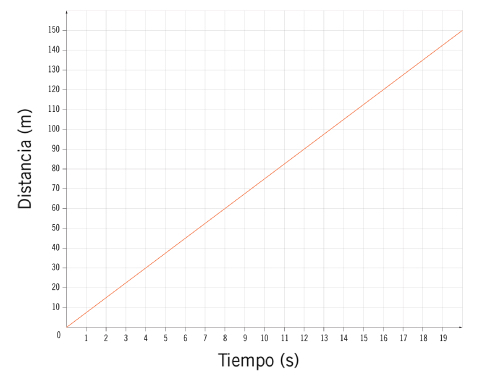
\includegraphics[width=0.5\textwidth]{../images/SINMAT1_U3_AC75_IMG2.jpg}
        \caption{Gráfica de la velocidad de un corredor.}
        \label{fig:SINMAT1_U3_AC75_IMG2}
    \end{figure}
    \begin{parts}
        \include*{../parts/question075b01}
        \include*{../parts/question075b02}
        \include*{../parts/question075b03}
        \include*{../parts/question075b04}
        \include*{../parts/question075b05}
    \end{parts}
\end{multicols}